\section{October 9, 2026}
% Based on pages 14--16 of 6-7-week.pdf.

We construct Adams--Bashforth and Adams--Moulton methods by integrating
polynomial interpolants. We then distinguish their automatic
zero-stability from absolute stability on \(x'=\lambda x\).
As before, \(t_n=t_0+n\tau\), \(f_n=f(t_n,x_n)\), and \(\tau>0\)
is constant.

\subsection{Adams formulas as quadrature rules}

An Adams method has the form
\begin{equation}\label{eq:adams-oct-09}
 x_{n+k}-x_{n+k-1}=\tau\sum_{j=0}^k\beta_jf_{n+j}.
\end{equation}
Its first characteristic polynomial is
\[
 \rho(\zeta)=\zeta^{k-1}(\zeta-1).
\]
Hence it satisfies the root condition for every \(k\): one is a
simple root, and all other roots lie strictly inside the unit disk.
This proves zero-stability, regardless of the quadrature weights.

The exact solution satisfies
\[
 x(t_{n+k})-x(t_{n+k-1})
      =\int_{t_{n+k-1}}^{t_{n+k}}x'(t)\,dt.
\]
Thus its residual in \eqref{eq:adams-oct-09} is the quadrature error
\begin{equation}\label{eq:adams-quadrature-error-oct-09}
 \mathcal L_\tau[x](t_n)
  =\int_{t_{n+k-1}}^{t_{n+k}}x'(t)\,dt
       -\tau\sum_{j=0}^k\beta_jx'(t_{n+j}).
\end{equation}
This is the same interpolation-and-integration principle used for
collocation, but most of the derivative samples now come from
previous steps.

Normalize time relative to the new endpoint:
\[
 t=t_{n+k}+\tau\theta,\qquad -1\leq\theta\leq0,
 \qquad v(\theta)=x'(t_{n+k}+\tau\theta).
\]
The sample at \(t_{n+j}\) has node \(\theta_j=j-k\).
Given a set \(J\) of sample indices, form the Lagrange basis
\[
 \ell_j(\theta)
   =\prod_{\substack{m\in J\\m\neq j}}
        \frac{\theta-\theta_m}{\theta_j-\theta_m},
 \qquad j\in J.
\]
Integrating the interpolant gives the weights
\begin{equation}\label{eq:adams-weights-oct-09}
 \boxed{\beta_j=\int_{-1}^0\ell_j(\theta)\,d\theta
           \quad(j\in J),}
\end{equation}
with zero weights for omitted samples. In particular, the weights
sum to one because the basis functions sum to one. This verifies
the consistency condition \(\sigma(1)=\rho'(1)=1\).

\subsection{Adams--Bashforth: extrapolating known derivatives}

For the \(k\)-step Adams--Bashforth method (AB\(k\)), use only
\(j=0,\ldots,k-1\), so the nodes are \(-k,\ldots,-1\).
The interpolant has degree at most \(k-1\), and \(\beta_k=0\).
The formula is explicit because all derivative values are known.
Its use over \([-1,0]\) extrapolates the derivative beyond the last
known sample.

The interpolation error contains \(k\) time differences and the
integration contributes one more power of \(\tau\). Therefore
\[
 \mathcal L_\tau[x](t_n)=O(\tau^{k+1}).
\]
The order is exactly \(k\): for the first omitted monomial,
the interpolation remainder is proportional to
\(\prod_{m=1}^k(\theta+m)\), whose integral on \([-1,0]\)
is strictly positive. Since Adams methods are zero-stable,
AB\(k\) converges with order \(k\) when initialized accurately
enough.

The first three formulas from class are
\begin{align}
 \text{AB1:}\qquad
 x_{n+1}-x_n&=\tau f_n,
       \label{eq:ab1-oct-09}\\
 \text{AB2:}\qquad
 x_{n+2}-x_{n+1}&=\tau\left(\frac32f_{n+1}-\frac12f_n\right),
       \label{eq:ab2-oct-09}\\
 \text{AB3:}\qquad
 x_{n+3}-x_{n+2}&=\tau\left(\frac{23}{12}f_{n+2}
                  -\frac{16}{12}f_{n+1}+\frac5{12}f_n\right).
       \label{eq:ab3-oct-09}
\end{align}
AB1 is forward Euler. For AB2, the basis functions at the nodes
\(-2,-1\) are \(\ell_0(\theta)=-\theta-1\) and
\(\ell_1(\theta)=\theta+2\); their integrals are \(-1/2\)
and \(3/2\), respectively.

For comparison with the fourth-order stability curve sketched in
class, the same construction gives
\begin{equation}\label{eq:ab4-oct-09}
 x_{n+4}-x_{n+3}
   =\frac\tau{24}\bigl(55f_{n+3}-59f_{n+2}+37f_{n+1}-9f_n\bigr).
\end{equation}
The leading residuals, expanded about \(t_n\), are
\[
 \begin{array}{c|c|c}
  \text{method}&p&\mathcal L_\tau[x](t_n)\\ \hline
  \text{AB1}&1&\tfrac12\tau^2x''(t_n)+O(\tau^3)\\
  \text{AB2}&2&\tfrac5{12}\tau^3x'''(t_n)+O(\tau^4)\\
  \text{AB3}&3&\tfrac38\tau^4x^{(4)}(t_n)+O(\tau^5)\\
  \text{AB4}&4&\tfrac{251}{720}\tau^5x^{(5)}(t_n)+O(\tau^6)
 \end{array}.
\]

\subsection{Stored derivatives and cost per step}

After initialization, AB\(k\) retains the latest \(k\) derivative
values. It forms the new solution by a weighted sum, evaluates
\(f\) once at that new solution, and discards the oldest derivative.
Thus it needs only one new function evaluation per step, independent
of \(k\). For example, AB3 uses one new evaluation per step,
whereas a standard three-stage third-order explicit RK method uses
three. The saving comes with storage, startup requirements, and
different stability restrictions. If the time step changes, the
interpolation nodes and hence the weights generally change too.

\subsection{Adams--Moulton: including the new endpoint}

For the implicit Adams--Moulton construction in the indexing
\eqref{eq:adams-oct-09}, take \(J=\{0,\ldots,k\}\): the nodes are
\(-k,\ldots,0\), and the interpolant has degree at most \(k\).
Now \(\beta_k\neq0\), so an implicit equation must be solved for
\(x_{n+k}\). The residual is \(O(\tau^{k+2})\), and the method
has order \(k+1\). The first omitted interpolation remainder has
one sign on \((-1,0)\), showing that this order is exact.

For example, nodes \(-1,0\) give the trapezoidal method
\[
 x_{n+1}-x_n=\frac\tau2(f_n+f_{n+1}),
 \qquad p=2,
\]
and nodes \(-2,-1,0\) give
\begin{equation}\label{eq:am3-oct-09}
 x_{n+2}-x_{n+1}
    =\tau\left(-\frac1{12}f_n+\frac8{12}f_{n+1}
                              +\frac5{12}f_{n+2}\right),
 \qquad p=3.
\end{equation}
Backward Euler is the first-order member of the Adams--Moulton
family, using only the new endpoint derivative. Names such as
``AM3'' often refer to order rather than number of steps; here we
state both the formula and its order to avoid this ambiguity.

An Adams--Bashforth prediction can provide an initial guess for the
implicit solve. Using a finite number of correction sweeps instead
of solving the Adams--Moulton equation defines a predictor--corrector
algorithm whose stability must be analyzed as that actual algorithm.

\subsection{Absolute stability of a general LMM}

On the scalar test equation \(x'=\lambda x\), with
\(z=\tau\lambda\), a general LMM becomes
\[
 \rho(E)x_n=z\sigma(E)x_n.
\]
Trying a mode \(x_n=\zeta^n\) gives the stability polynomial
\begin{equation}\label{eq:lmm-stability-polynomial-oct-09}
 \boxed{\pi_z(\zeta)=\rho(\zeta)-z\sigma(\zeta)=0.}
\end{equation}
For a genuine \(k\)-step recurrence we require
\(\alpha_k-z\beta_k\neq0\), so the new value is uniquely
determined from the history. Unlike the RK test equation, there
are generally \(k\) amplification modes, rather than a single
stability factor \(R(z)\).

Following the convention used for RK methods, define
\begin{align*}
 \mathcal S&=\{z:\alpha_k-z\beta_k\neq0,
              \text{ all roots of }\pi_z\text{ have }|\zeta|<1\},\\
 \mathcal D&=\{z:\alpha_k-z\beta_k\neq0,
              \pi_z\text{ satisfies the root condition}\}.
\end{align*}
The first set gives decay of every numerical solution; the second
gives boundedness for every initial history. At \(z=0\), this is
exactly zero-stability. A consistent zero-stable method has a simple
root at \(\zeta=1\), so \(0\in\mathcal D\) but
\(0\notin\mathcal S\).

A candidate boundary is obtained by putting a root on the unit
circle:
\begin{equation}\label{eq:lmm-boundary-oct-09}
 z(\theta)=\frac{\rho(e^{i\theta})}{\sigma(e^{i\theta})},
 \qquad 0\leq\theta\leq2\pi,
\end{equation}
where the denominator is nonzero. This is the boundary-locus
construction. All the other roots must still be checked: a traced
curve need not consist entirely of the boundary of \(\mathcal D\).

\subsection{The stability restriction for AB2}

Substituting \(f_n=\lambda x_n\) into AB2 gives
\[
 x_{n+2}-\left(1+\frac32z\right)x_{n+1}
                   +\frac12z\,x_n=0.
\]
Thus
\begin{equation}\label{eq:ab2-stability-oct-09}
 \pi_z(\zeta)=\zeta^2-\left(1+\frac32z\right)\zeta+\frac12z,
 \qquad
 \rho(\zeta)=\zeta^2-\zeta,\quad
 \sigma(\zeta)=\frac32\zeta-\frac12.
\end{equation}
Its roots are
\[
 \zeta_\pm(z)=\frac{1+3z/2
              \ \pm\sqrt{(1+3z/2)^2-2z}}2.
\]
Near zero, one root approximates the physical mode
\(\zeta_+(z)=1+z+O(z^2)\), and the other satisfies
\(\zeta_-(z)=z/2+O(z^2)\).

For real \(z<0\), the discriminant
\(1+z+9z^2/4\) is positive and the root product \(z/2\) is
negative. Write the roots as \(\zeta_-<0<\zeta_+\).
Since
\[
 \pi_z(1)=-z>0,\qquad \pi_z(-1)=2+2z,
\]
the positive root lies below one, and the negative root lies above
minus one exactly when \(z>-1\). Hence
\begin{equation}\label{eq:ab2-real-interval-oct-09}
 \boxed{\mathcal S\cap\bb R=(-1,0),\qquad
        \mathcal D\cap\bb R=[-1,0].}
\end{equation}
For \(z>0\), \(\pi_z(1)<0\) forces a root larger than one.
At \(z=-1\), the roots are \(-1\) and \(1/2\): the iterates
are bounded, but an alternating component does not decay.
For a negative real \(\lambda\), strict decay therefore requires
\(0<\tau<1/|\lambda|\).

The same polynomial test yields the negative real intervals
\[
 \begin{array}{c|c|c}
  \text{method}&\mathcal S\cap\bb R&\mathcal D\cap\bb R\\ \hline
  \text{AB1}&(-2,0)&[-2,0]\\
  \text{AB2}&(-1,0)&[-1,0]\\
  \text{AB3}&(-6/11,0)&[-6/11,0]\\
  \text{AB4}&(-3/10,0)&[-3/10,0]
 \end{array}.
\]
In each case the left endpoint is reached when a root passes through
\(\zeta=-1\), so it equals \(\rho(-1)/\sigma(-1)\).
The other roots satisfy the root condition there. These intervals
illustrate the shrinking tolerance for negative real modes as the
AB order increases. Zero-stability of every Adams method guarantees
control in the small-step convergence limit; it does not remove
the absolute-stability restriction at a chosen finite step.

\begin{figure}[!htbp]
\centering
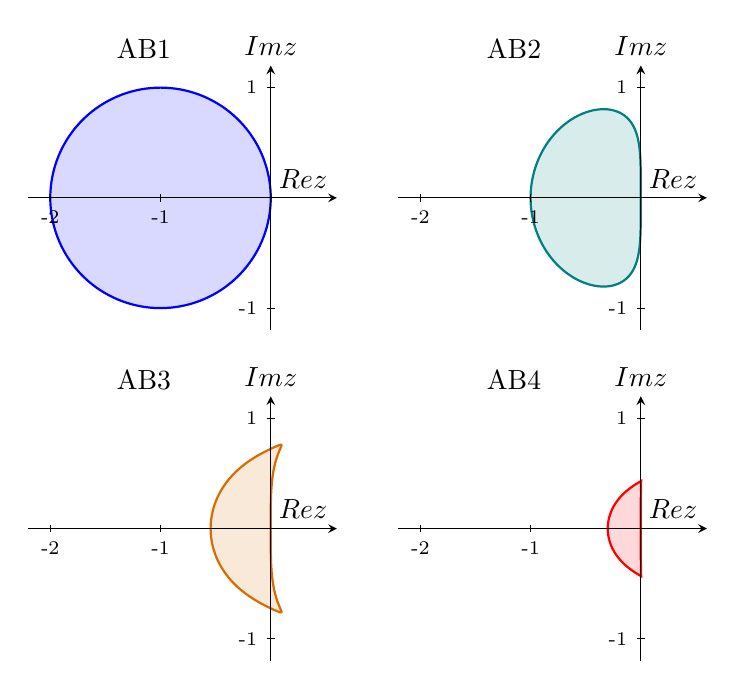
\begin{tikzpicture}[>=stealth]
% Boundary loci rho(exp(i theta))/sigma(exp(i theta)).
% For AB4, retain only arcs on which every other root is in the disk.
% Its intersecting branches meet at theta = 0.42786387, 2.02542712.
\begin{scope}[xshift=0cm,yshift=0cm,xscale=1.4,yscale=1.4]
\filldraw[fill=blue!15,draw=blue,thick] plot coordinates {
(0.000000,0.000000) (-0.001007,0.044865) (-0.004026,0.089639) (-0.009050,0.134233) (-0.016070,0.178557)
(-0.025072,0.222521) (-0.036037,0.266037) (-0.048943,0.309017) (-0.063765,0.351375) (-0.080472,0.393025)
(-0.099031,0.433884) (-0.119404,0.473869) (-0.141551,0.512899) (-0.165427,0.550897) (-0.190983,0.587785)
(-0.218169,0.623490) (-0.246929,0.657939) (-0.277205,0.691063) (-0.308937,0.722795) (-0.342061,0.753071)
(-0.376510,0.781831) (-0.412215,0.809017) (-0.449103,0.834573) (-0.487101,0.858449) (-0.526131,0.880596)
(-0.566116,0.900969) (-0.606975,0.919528) (-0.648625,0.936235) (-0.690983,0.951057) (-0.733963,0.963963)
(-0.777479,0.974928) (-0.821443,0.983930) (-0.865767,0.990950) (-0.910361,0.995974) (-0.955135,0.998993)
(-1.000000,1.000000) (-1.044865,0.998993) (-1.089639,0.995974) (-1.134233,0.990950) (-1.178557,0.983930)
(-1.222521,0.974928) (-1.266037,0.963963) (-1.309017,0.951057) (-1.351375,0.936235) (-1.393025,0.919528)
(-1.433884,0.900969) (-1.473869,0.880596) (-1.512899,0.858449) (-1.550897,0.834573) (-1.587785,0.809017)
(-1.623490,0.781831) (-1.657939,0.753071) (-1.691063,0.722795) (-1.722795,0.691063) (-1.753071,0.657939)
(-1.781831,0.623490) (-1.809017,0.587785) (-1.834573,0.550897) (-1.858449,0.512899) (-1.880596,0.473869)
(-1.900969,0.433884) (-1.919528,0.393025) (-1.936235,0.351375) (-1.951057,0.309017) (-1.963963,0.266037)
(-1.974928,0.222521) (-1.983930,0.178557) (-1.990950,0.134233) (-1.995974,0.089639) (-1.998993,0.044865)
(-2.000000,0.000000) (-1.998993,-0.044865) (-1.995974,-0.089639) (-1.990950,-0.134233) (-1.983930,-0.178557)
(-1.974928,-0.222521) (-1.963963,-0.266037) (-1.951057,-0.309017) (-1.936235,-0.351375) (-1.919528,-0.393025)
(-1.900969,-0.433884) (-1.880596,-0.473869) (-1.858449,-0.512899) (-1.834573,-0.550897) (-1.809017,-0.587785)
(-1.781831,-0.623490) (-1.753071,-0.657939) (-1.722795,-0.691063) (-1.691063,-0.722795) (-1.657939,-0.753071)
(-1.623490,-0.781831) (-1.587785,-0.809017) (-1.550897,-0.834573) (-1.512899,-0.858449) (-1.473869,-0.880596)
(-1.433884,-0.900969) (-1.393025,-0.919528) (-1.351375,-0.936235) (-1.309017,-0.951057) (-1.266037,-0.963963)
(-1.222521,-0.974928) (-1.178557,-0.983930) (-1.134233,-0.990950) (-1.089639,-0.995974) (-1.044865,-0.998993)
(-1.000000,-1.000000) (-0.955135,-0.998993) (-0.910361,-0.995974) (-0.865767,-0.990950) (-0.821443,-0.983930)
(-0.777479,-0.974928) (-0.733963,-0.963963) (-0.690983,-0.951057) (-0.648625,-0.936235) (-0.606975,-0.919528)
(-0.566116,-0.900969) (-0.526131,-0.880596) (-0.487101,-0.858449) (-0.449103,-0.834573) (-0.412215,-0.809017)
(-0.376510,-0.781831) (-0.342061,-0.753071) (-0.308937,-0.722795) (-0.277205,-0.691063) (-0.246929,-0.657939)
(-0.218169,-0.623490) (-0.190983,-0.587785) (-0.165427,-0.550897) (-0.141551,-0.512899) (-0.119404,-0.473869)
(-0.099031,-0.433884) (-0.080472,-0.393025) (-0.063765,-0.351375) (-0.048943,-0.309017) (-0.036037,-0.266037)
(-0.025072,-0.222521) (-0.016070,-0.178557) (-0.009050,-0.134233) (-0.004026,-0.089639) (-0.001007,-0.044865)
(0.000000,-0.000000)
} -- cycle;
 \draw[->] (-2.2,0)--(.6,0) node[above left] {\(\operatorname{Re}z\)};
 \draw[->] (0,-1.2)--(0,1.2) node[above] {\(\operatorname{Im}z\)};
 \foreach \x in {-2,-1}
  \draw (\x,.035)--(\x,-.035) node[below] {\scriptsize \x};
 \foreach \y in {-1,1}
  \draw (.035,\y)--(-.035,\y) node[left] {\scriptsize \y};
 \node at (-1.15,1.35) {AB1};
\end{scope}
\begin{scope}[xshift=4.7cm,yshift=0cm,xscale=1.4,yscale=1.4]
\filldraw[fill=teal!15,draw=teal,thick] plot coordinates {
(0.000000,0.000000) (-0.000001,0.044842) (-0.000016,0.089460) (-0.000081,0.133634) (-0.000252,0.177156)
(-0.000606,0.219833) (-0.001232,0.261489) (-0.002232,0.301972) (-0.003711,0.341150) (-0.005778,0.378914)
(-0.008539,0.415178) (-0.012092,0.449875) (-0.016528,0.482956) (-0.021925,0.514389) (-0.028352,0.544156)
(-0.035862,0.572246) (-0.044494,0.598662) (-0.054275,0.623410) (-0.065219,0.646501) (-0.077329,0.667949)
(-0.090595,0.687770) (-0.104998,0.705982) (-0.120511,0.722600) (-0.137097,0.737641) (-0.154714,0.751122)
(-0.173314,0.763055) (-0.192843,0.773456) (-0.213243,0.782336) (-0.234453,0.789708) (-0.256409,0.795583)
(-0.279046,0.799972) (-0.302293,0.802885) (-0.326084,0.804333) (-0.350345,0.804328) (-0.375008,0.802879)
(-0.400000,0.800000) (-0.425250,0.795703) (-0.450686,0.790002) (-0.476238,0.782912) (-0.501835,0.774449)
(-0.527407,0.764631) (-0.552887,0.753478) (-0.578205,0.741011) (-0.603296,0.727253) (-0.628094,0.712227)
(-0.652535,0.695962) (-0.676556,0.678484) (-0.700098,0.659824) (-0.723100,0.640015) (-0.745506,0.619090)
(-0.767260,0.597085) (-0.788309,0.574038) (-0.808601,0.549989) (-0.828087,0.524978) (-0.846720,0.499049)
(-0.864455,0.472247) (-0.881250,0.444618) (-0.897064,0.416209) (-0.911861,0.387070) (-0.925605,0.357253)
(-0.938265,0.326807) (-0.949809,0.295788) (-0.960212,0.264248) (-0.969448,0.232244) (-0.977497,0.199831)
(-0.984340,0.167067) (-0.989960,0.134008) (-0.994345,0.100713) (-0.997484,0.067241) (-0.999371,0.033650)
(-1.000000,0.000000) (-0.999371,-0.033650) (-0.997484,-0.067241) (-0.994345,-0.100713) (-0.989960,-0.134008)
(-0.984340,-0.167067) (-0.977497,-0.199831) (-0.969448,-0.232244) (-0.960212,-0.264248) (-0.949809,-0.295788)
(-0.938265,-0.326807) (-0.925605,-0.357253) (-0.911861,-0.387070) (-0.897064,-0.416209) (-0.881250,-0.444618)
(-0.864455,-0.472247) (-0.846720,-0.499049) (-0.828087,-0.524978) (-0.808601,-0.549989) (-0.788309,-0.574038)
(-0.767260,-0.597085) (-0.745506,-0.619090) (-0.723100,-0.640015) (-0.700098,-0.659824) (-0.676556,-0.678484)
(-0.652535,-0.695962) (-0.628094,-0.712227) (-0.603296,-0.727253) (-0.578205,-0.741011) (-0.552887,-0.753478)
(-0.527407,-0.764631) (-0.501835,-0.774449) (-0.476238,-0.782912) (-0.450686,-0.790002) (-0.425250,-0.795703)
(-0.400000,-0.800000) (-0.375008,-0.802879) (-0.350345,-0.804328) (-0.326084,-0.804333) (-0.302293,-0.802885)
(-0.279046,-0.799972) (-0.256409,-0.795583) (-0.234453,-0.789708) (-0.213243,-0.782336) (-0.192843,-0.773456)
(-0.173314,-0.763055) (-0.154714,-0.751122) (-0.137097,-0.737641) (-0.120511,-0.722600) (-0.104998,-0.705982)
(-0.090595,-0.687770) (-0.077329,-0.667949) (-0.065219,-0.646501) (-0.054275,-0.623410) (-0.044494,-0.598662)
(-0.035862,-0.572246) (-0.028352,-0.544156) (-0.021925,-0.514389) (-0.016528,-0.482956) (-0.012092,-0.449875)
(-0.008539,-0.415178) (-0.005778,-0.378914) (-0.003711,-0.341150) (-0.002232,-0.301972) (-0.001232,-0.261489)
(-0.000606,-0.219833) (-0.000252,-0.177156) (-0.000081,-0.133634) (-0.000016,-0.089460) (-0.000001,-0.044842)
(0.000000,-0.000000)
} -- cycle;
 \draw[->] (-2.2,0)--(.6,0) node[above left] {\(\operatorname{Re}z\)};
 \draw[->] (0,-1.2)--(0,1.2) node[above] {\(\operatorname{Im}z\)};
 \foreach \x in {-2,-1}
  \draw (\x,.035)--(\x,-.035) node[below] {\scriptsize \x};
 \foreach \y in {-1,1}
  \draw (.035,\y)--(-.035,\y) node[left] {\scriptsize \y};
 \node at (-1.15,1.35) {AB2};
\end{scope}
\begin{scope}[xshift=0cm,yshift=-4.2cm,xscale=1.4,yscale=1.4]
\filldraw[fill=orange!85!black!15,draw=orange!85!black,thick] plot coordinates {
(0.000000,0.000000) (0.000002,0.044880) (0.000024,0.089757) (0.000122,0.134622) (0.000381,0.179445)
(0.000919,0.224170) (0.001873,0.268710) (0.003400,0.312930) (0.005654,0.356648) (0.008781,0.399631)
(0.012901,0.441591) (0.018085,0.482194) (0.024344,0.521069) (0.031612,0.557827) (0.039737,0.592086)
(0.048481,0.623492) (0.057529,0.651754) (0.066509,0.676659) (0.075013,0.698093) (0.082630,0.716047)
(0.088975,0.730608) (0.093712,0.741953) (0.096576,0.750320) (0.097378,0.755991) (0.096009,0.759267)
(0.092433,0.760447) (0.086681,0.759814) (0.078835,0.757622) (0.069014,0.754093) (0.057369,0.749411)
(0.044062,0.743725) (0.029267,0.737155) (0.013158,0.729787) (-0.004094,0.721686) (-0.022325,0.712897)
(-0.041379,0.703448) (-0.061110,0.693356) (-0.081382,0.682629) (-0.102067,0.671267) (-0.123049,0.659268)
(-0.144219,0.646626) (-0.165477,0.633335) (-0.186729,0.619389) (-0.207890,0.604782) (-0.228880,0.589511)
(-0.249624,0.573572) (-0.270053,0.556967) (-0.290101,0.539698) (-0.309709,0.521769) (-0.328819,0.503189)
(-0.347379,0.483968) (-0.365337,0.464118) (-0.382647,0.443655) (-0.399265,0.422597) (-0.415149,0.400962)
(-0.430261,0.378775) (-0.444565,0.356058) (-0.458028,0.332839) (-0.470617,0.309145) (-0.482305,0.285007)
(-0.493064,0.260455) (-0.502872,0.235522) (-0.511705,0.210244) (-0.519545,0.184655) (-0.526374,0.158792)
(-0.532178,0.132692) (-0.536944,0.106393) (-0.540661,0.079935) (-0.543322,0.053357) (-0.544921,0.026699)
(-0.545455,0.000000) (-0.544921,-0.026699) (-0.543322,-0.053357) (-0.540661,-0.079935) (-0.536944,-0.106393)
(-0.532178,-0.132692) (-0.526374,-0.158792) (-0.519545,-0.184655) (-0.511705,-0.210244) (-0.502872,-0.235522)
(-0.493064,-0.260455) (-0.482305,-0.285007) (-0.470617,-0.309145) (-0.458028,-0.332839) (-0.444565,-0.356058)
(-0.430261,-0.378775) (-0.415149,-0.400962) (-0.399265,-0.422597) (-0.382647,-0.443655) (-0.365337,-0.464118)
(-0.347379,-0.483968) (-0.328819,-0.503189) (-0.309709,-0.521769) (-0.290101,-0.539698) (-0.270053,-0.556967)
(-0.249624,-0.573572) (-0.228880,-0.589511) (-0.207890,-0.604782) (-0.186729,-0.619389) (-0.165477,-0.633335)
(-0.144219,-0.646626) (-0.123049,-0.659268) (-0.102067,-0.671267) (-0.081382,-0.682629) (-0.061110,-0.693356)
(-0.041379,-0.703448) (-0.022325,-0.712897) (-0.004094,-0.721686) (0.013158,-0.729787) (0.029267,-0.737155)
(0.044062,-0.743725) (0.057369,-0.749411) (0.069014,-0.754093) (0.078835,-0.757622) (0.086681,-0.759814)
(0.092433,-0.760447) (0.096009,-0.759267) (0.097378,-0.755991) (0.096576,-0.750320) (0.093712,-0.741953)
(0.088975,-0.730608) (0.082630,-0.716047) (0.075013,-0.698093) (0.066509,-0.676659) (0.057529,-0.651754)
(0.048481,-0.623492) (0.039737,-0.592086) (0.031612,-0.557827) (0.024344,-0.521069) (0.018085,-0.482194)
(0.012901,-0.441591) (0.008781,-0.399631) (0.005654,-0.356648) (0.003400,-0.312930) (0.001873,-0.268710)
(0.000919,-0.224170) (0.000381,-0.179445) (0.000122,-0.134622) (0.000024,-0.089757) (0.000002,-0.044880)
(0.000000,-0.000000)
} -- cycle;
 \draw[->] (-2.2,0)--(.6,0) node[above left] {\(\operatorname{Re}z\)};
 \draw[->] (0,-1.2)--(0,1.2) node[above] {\(\operatorname{Im}z\)};
 \foreach \x in {-2,-1}
  \draw (\x,.035)--(\x,-.035) node[below] {\scriptsize \x};
 \foreach \y in {-1,1}
  \draw (.035,\y)--(-.035,\y) node[left] {\scriptsize \y};
 \node at (-1.15,1.35) {AB3};
\end{scope}
\begin{scope}[xshift=4.7cm,yshift=-4.2cm,xscale=1.4,yscale=1.4]
\filldraw[fill=red!15,draw=red,thick] plot coordinates {
(0.000000,0.000000) (0.000000,0.022519) (0.000000,0.045038) (0.000000,0.067558) (0.000000,0.090079)
(0.000001,0.112602) (0.000003,0.135130) (0.000008,0.157667) (0.000018,0.180217) (0.000037,0.202785)
(0.000069,0.225380) (0.000122,0.248010) (0.000204,0.270685) (0.000328,0.293417) (0.000508,0.316218)
(0.000764,0.339101) (0.001119,0.362080) (0.001600,0.385170) (0.002240,0.408383) (0.003077,0.431733)
(0.003077,0.431733) (-0.008448,0.425133) (-0.019774,0.418476) (-0.030901,0.411756) (-0.041825,0.404965)
(-0.052544,0.398099) (-0.063058,0.391151) (-0.073364,0.384118) (-0.083461,0.376995) (-0.093346,0.369780)
(-0.103020,0.362469) (-0.112479,0.355060) (-0.121723,0.347553) (-0.130750,0.339945) (-0.139558,0.332235)
(-0.148146,0.324423) (-0.156513,0.316509) (-0.164657,0.308493) (-0.172577,0.300375) (-0.180271,0.292157)
(-0.187738,0.283838) (-0.194976,0.275421) (-0.201984,0.266907) (-0.208760,0.258298) (-0.215304,0.249594)
(-0.221613,0.240800) (-0.227687,0.231916) (-0.233524,0.222945) (-0.239122,0.213890) (-0.244482,0.204753)
(-0.249601,0.195538) (-0.254478,0.186247) (-0.259112,0.176884) (-0.263502,0.167451) (-0.267647,0.157952)
(-0.271546,0.148391) (-0.275198,0.138770) (-0.278602,0.129095) (-0.281758,0.119367) (-0.284664,0.109591)
(-0.287320,0.099771) (-0.289725,0.089910) (-0.291879,0.080013) (-0.293780,0.070083) (-0.295429,0.060125)
(-0.296825,0.050142) (-0.297968,0.040138) (-0.298857,0.030118) (-0.299492,0.020085) (-0.299873,0.010045)
(-0.300000,0.000000) (-0.299873,-0.010045) (-0.299492,-0.020085) (-0.298857,-0.030118) (-0.297968,-0.040138)
(-0.296825,-0.050142) (-0.295429,-0.060125) (-0.293780,-0.070083) (-0.291879,-0.080013) (-0.289725,-0.089910)
(-0.287320,-0.099771) (-0.284664,-0.109591) (-0.281758,-0.119367) (-0.278602,-0.129095) (-0.275198,-0.138770)
(-0.271546,-0.148391) (-0.267647,-0.157952) (-0.263502,-0.167451) (-0.259112,-0.176884) (-0.254478,-0.186247)
(-0.249601,-0.195538) (-0.244482,-0.204753) (-0.239122,-0.213890) (-0.233524,-0.222945) (-0.227687,-0.231916)
(-0.221613,-0.240800) (-0.215304,-0.249594) (-0.208760,-0.258298) (-0.201984,-0.266907) (-0.194976,-0.275421)
(-0.187738,-0.283838) (-0.180271,-0.292157) (-0.172577,-0.300375) (-0.164657,-0.308493) (-0.156513,-0.316509)
(-0.148146,-0.324423) (-0.139558,-0.332235) (-0.130750,-0.339945) (-0.121723,-0.347553) (-0.112479,-0.355060)
(-0.103020,-0.362469) (-0.093346,-0.369780) (-0.083461,-0.376995) (-0.073364,-0.384118) (-0.063058,-0.391151)
(-0.052544,-0.398099) (-0.041825,-0.404965) (-0.030901,-0.411756) (-0.019774,-0.418476) (-0.008448,-0.425133)
(0.003077,-0.431733) (0.003077,-0.431733) (0.002240,-0.408383) (0.001600,-0.385170) (0.001119,-0.362080)
(0.000764,-0.339101) (0.000508,-0.316218) (0.000328,-0.293417) (0.000204,-0.270685) (0.000122,-0.248010)
(0.000069,-0.225380) (0.000037,-0.202785) (0.000018,-0.180217) (0.000008,-0.157667) (0.000003,-0.135130)
(0.000001,-0.112602) (0.000000,-0.090079) (0.000000,-0.067558) (0.000000,-0.045038) (0.000000,-0.022519)
(0.000000,-0.000000)
} -- cycle;
 \draw[->] (-2.2,0)--(.6,0) node[above left] {\(\operatorname{Re}z\)};
 \draw[->] (0,-1.2)--(0,1.2) node[above] {\(\operatorname{Im}z\)};
 \foreach \x in {-2,-1}
  \draw (\x,.035)--(\x,-.035) node[below] {\scriptsize \x};
 \foreach \y in {-1,1}
  \draw (.035,\y)--(-.035,\y) node[left] {\scriptsize \y};
 \node at (-1.15,1.35) {AB4};
\end{scope}
\end{tikzpicture}
\caption{Computed stability domains for the first four Adams--Bashforth
methods on the same scale. Shading indicates the root condition.
For AB4, only the stable parts of the boundary locus are retained.}
\label{fig:adams-domains-oct-09}
\end{figure}
